% ---- Modele TP PC V2 -----------
\documentclass[a4paper,10pt,french]{scrartcl}
\usepackage[T1]{fontenc}%---pour l'encodage d'entr\'ee
\usepackage{array}%---pour les tableaux
\usepackage{titlesec}%---modification des titres
\usepackage{ulem}%---pour le soulignage
\usepackage[dvipsnames]{xcolor}%---pour avoir d'autres couleurs
\usepackage{color}%---pour avoir les couleurs de base
\usepackage{babel}%---pour les trucs de langue et la francasation

\usepackage{graphicx}%----pour mettre des images
\usepackage[utf8]{inputenc}%---encodage
\usepackage{geometry}%---pour modifier les tailles et mettre a4paper
%\usepackage{awesomebox}%---pour les boites d'exercices, de pbq et de croquis ---d\'esactiv\'e pour les TP de PC
\usepackage{tikz}%---pour dessiner + d\'ependance de chemfig
\usepackage{chemfig}%---pour dessiner formules chimiques
\usepackage{chemformula}%---pour les formules chimiques en \'equation : \ch{...}
\usepackage{tabularx}%---pour dimensionner automatiquement les tableaux avec variable X
\usepackage{awesomebox}%---Pour les boites info, danger et autres
\usepackage{fancyhdr}%---pour les en-t\^ete personnalis\'ees
\usepackage{blindtext}%---pour les liens
\usepackage{hyperref}%---pour les liens (\`a mettre en dernier)
\usepackage{caption}%---pour la francisation de la l\'egende table vers Tableau
 \usepackage{float}

\captionsetup{labelfont=sc}%---pour la francisation de la l\'egende table vers Tableau
\def\frenchtablename{Tableau}%---pour la francisation de la l\'egende table vers Tableau
\pagestyle{fancy}
\renewcommand\headrulewidth{1pt}
\fancyhead[L]{TP n°3}
\fancyhead[R]{Saux - Gadré-Dacheville}
\title{Compte rendu de TP N°3}
\date{}
\author{}

\geometry{a4paper}
% ----------- Création des commandes de couleur ----------
\makeatletter
\newcommand{\coloruline}[2]{%
        \UL@protected\def\temp@uline{\leavevmode \bgroup
            \markoverwith{\textcolor{#1}{\rule[-0.5ex]{2pt}{0.4pt}}}%
        \ULon}%
        \temp@uline{#2}%
    }

    \newcommand{\coloruuline}[2]{%
        \UL@protected\def\temp@uuline{\leavevmode \bgroup
            \UL@setULdepth
            \ifx\UL@on\UL@onin \advance\ULdepth2.8\p@\fi
            \markoverwith{\textcolor{#1}{\lower\ULdepth\hbox
                {\kern-.03em\vbox{\hrule width.2em\kern1\p@\hrule}\kern-.03em}}}%
        \ULon}%
        \temp@uuline{#2}%
    }

    \newcommand{\coloruwave}[2]{%
        \UL@protected\def\temp@uwave{\leavevmode \bgroup
        \ifdim \ULdepth=\maxdimen \ULdepth 3.5\p@
        \else \advance\ULdepth2\p@
        \fi \markoverwith{\textcolor{#1}{\lower\ULdepth\hbox{\sixly \char58}}}\ULon}
        \font\sixly=lasy6 % does not re-load if already loaded, so no memory drain.
        \temp@uwave{#2}%
    }
\makeatother

\renewcommand{\thesection}{\arabic{section}}
\renewcommand{\thesubsection}{\arabic{subsection}}
\renewcommand{\thesubsubsection}{\arabic{subsubsection}}
\begin{document}
% ---------------- Modification des titres de niveau 1,2 et 3 --------------------
\titleformat
{\section} % command
%[display] % shape
{\Large} % format
{\coloruuline{red}{\thesection. }} % label
{0ex} % sep
{\coloruuline{red}} % before-code
[] % after-code

\titleformat
{\subsection} % command
%[display] % shape
{\Large} % format
{\coloruline{red}{\thesection.\thesubsection. }} % label
{0ex} % sep
{\coloruline{red}} % before-code
[] % after-code

\titleformat
{\subsubsection} % command
%[display] % shape
{\large} % format
{\coloruline{ForestGreen}{\thesection.\thesubsection.\thesubsubsection. }} % label
{0ex} % sep
{\coloruline{ForestGreen}} % before-code
[] % after-code

\titleformat
{\chapter} % command
%[display] % shape
{\large} % format
{\coloruline{NavyBlue}{\thechapter \:- }} % label
{0ex} % sep
{\coloruline{NavyBlue}} % before-code
[] % after-code


% ---------------- Début du corps du document ------------------------------------
\section{Introduction}
L'objectif de ce TP est de déterminer la constante de raideur de trois ressorts différents. Pour ce faire nous utiliserons une approche dite 'statique' et une approche dite 'dynamique'. Ces deux approches doivent produire des résultats semblables et la comparaison des valeurs obtenues nous permettra de déterminer quelle méthode est la plus précise.
\section{Protocole}
Nous allons effectuer deux manipulations distinctes afin d'obtenir une valeur de deux façons.
\subsection{Approche statique}
\subsubsection{Matériel}
\begin{itemize}
 \item Le ressort dont on veut connaitre la constante de raideur
 \item Un index
 \item  Un support statif et une noix pour y fixer la réglette graduée et le ressort
 \item Une réglette graduée avec une graduation milimétrée
 \item Un support de masses fendues de 50g
 \item une masse fendue de 50 g
 \item 4 masses fendues de 100g
\end{itemize}

\subsubsection{Description du montage expérimental}
Nous fixons au support (1) le ressort (2) face à la règlette (3). Nous accrochons sur l'extrémitée libre l'index (4). À l'extrémité de celui-ci viendront se placer le support de masse (5), puis les masses (6), pour obtenir le montage représenté en figure \ref{fig1}.
\begin{figure}[H]
\begin{center}
 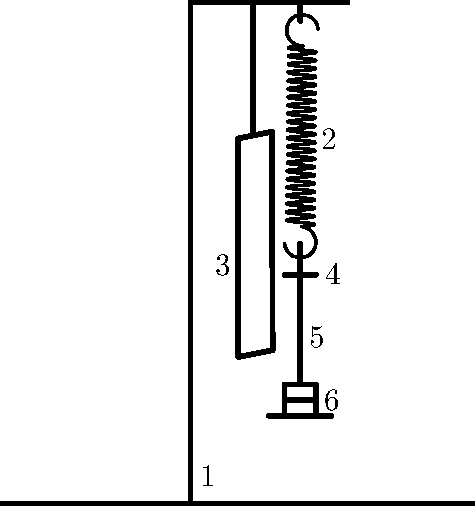
\includegraphics[scale=0.8]{path1}
 \end{center}
\caption{Montage expérimental de la première manipulation }
\label{fig1}
\end{figure}


\subsubsection{Mesures à effectuer}
Dans cette approche, nous allons obtenir la constante de raideur avec la mesure de l'alongement du ressort. Pour ce faire :
\begin{enumerate}
 \item Mesurer la position de l'index sur la règlette. Cette valeur est notée \(l_0\)
 \item Placer le support de masse fendues
 \item Placer les masses
 \item Attendre que le ressort se stabilise
 \item Mesurer la position de l'index. Cette valeur est notée \(x_i\)
 \item Répéter les étapes 3 à 5 avec différentes combinaisons de masse.
\end{enumerate}

\subsection{Approche dynamique}
\subsubsection{Matériel et description du montage expérimental}
Il s'agit du m\^eme montage expérimental que dans la partie précédente.
\subsubsection{Mesures à effectuer}
Dans cette approche, nous allons obtenir la constante de raideur avec la mesure de la période d'oscillation du ressort. Pour ce faire :
\begin{enumerate}
 \item Placer le support de masse fendues
 \item Placer les masses
 \item Tirer le ressort vers le bas sur quelques centimètres
 \item Relacher le ressort et commencer le chronomètrage en m\^eme temps.
 \item Lorsque le ressort a effectué 10 oscillations, arreter le chrnomètre et noter la valeur obtenue.
 \item Répéter les étapes 3 à 5 avec différentes combinaisons de masse.
\end{enumerate}
\section{Mesures}
\subsection{Approche statique}
On peut considérer l'incertitude sur les masses nulle mais la mesure de l'index apporte une incertitude de \(\frac{0.1}{\sqrt{3}}\) cm sur chaque mesure, car la plus petite graduation disponible était de 0.1 cm.

Les mesures effectuées sont synthétisées dans les tableaux suivants.
\begin{table}[H]
\begin{center}
 \begin{tabular}{lllllll}
Masse (g) & 0 & 50 &100&150&200&250\\
position de l'index (cm) & 3.8 & 3.9&6.8&10.1&13.5&16.9
\end{tabular}
\end{center}
\caption{Mesures effectuées avec le ressort 1}
\end{table}
\begin{table}[H]
\begin{center}
 \begin{tabular}{llllllll}
Masse (g) & 0 &50&100&200&250&300&350\\
position de l'index (cm) & 2.6 & 2.6&3.4&7.9&10.1&12.4&14.7
\end{tabular}
\end{center}
\caption{Mesures effectuées avec le ressort 2}
\end{table}
\begin{table}[H]
\begin{center}
 \begin{tabular}{llllllll}
Masse (g) & 0 &100&200&300&400&450&500\\
position de l'index (cm) & 2.2 & 2.3&4.2&6.8&9.4&10.7&12.0
\end{tabular}
\end{center}
\caption{Mesures effectuées avec le ressort 3}
\end{table}


\subsection{Approche dynamique}

\subsubsection{Données}
Ces mesures effectuées sont synthétisées dans les tableaux suivants :
\begin{table}[H]
\begin{center}
\begin{tabular}{lllll}
Masse (g) & 100 & 150 & 200 & 250\\
Temps (s) & 5.07 & 6.52 & 7.36 & 8.02\\
Temps (s) & 5.13 & 6.44 & 7.41 & 8.13\\
Temps (s) & 5.13 & 6.51 & 7.34 & 8.22\\
Temps (s) & 5.05 & 6.50 & 7.40 & 8.15
\end{tabular}
\end{center}
\caption{Mesures effectuées avec le ressort 1}
\end{table}
\begin{table}[H]
\begin{center}
\begin{tabular}{llllll}
Masse (g) & 150 & 200 & 250 & 300 & 350\\
Temps (s) & 5.06 & 5.83 & 6.41 & 7.13 & 7.77\\
Temps (s) & 5.05 & 5.87 & 6.53 & 7.12 & 7.71\\
Temps (s) & 5.05 & 5.98 & 6.59 & 7.11 & 7.70\\
Temps (s) & 5.10 & 5.89 & 6.55 & 7.16 & 7.87
\end{tabular}
\end{center}
\caption{Mesures effectuées avec le ressort 2}
\end{table}
\begin{table}[H]
\begin{center}
\begin{tabular}{llllll}
Masse (g) & 300 & 350 & 400 & 450 & 500\\
Temps (s) & 5.49 & 5.81 & 6.19 & 6.56 & 6.93\\
Temps (s) & 5.40 & 6.01 & 6.21 & 6.56 & 6.84\\
Temps (s) & 5.48 & 5.74 & 6.24 & 6.57 & 6.98\\
Temps (s) & 5.36 & 5.78 & 6.25 & 6.54 & 6.74
\end{tabular}
\caption{Mesures effectuées avec le ressort 3}
\end{center}
\end{table}
\subsubsection{Incertitude}
Pour diminier l'incertitude sur une période, nous avons mesuré le temps mis par la masse pour effectuer 10 périodes. Pour trouver le temps mis pour effectuer une période, il faut diviser le temps trouvé par 10.

On peut considérer l'incertitude de type B associée à la masse comme nulle. L'incertitude de type B associée à la mesure de temps de 10 périodes provient de la précision du chronomètre, ici au centième, du temps de réaction de l'expérimentateur ainsi que des oscillations du ressorts qui ne sont pas parfaitement verticales. Nous considérons que ces deux dernières sources d'incertitudes sont négligeables par rapport à l'incertitude liée à l'appareil de mesure qui est de \(\frac{0.026}{\sqrt{3}} = 0.015\).

L'incertitude liée à une période est alors de \(u_B(T_0) = \frac{u_B(T_{10})}{10} = \frac{0.015}{10} = 0.0015\).

Nous avons effectué dans chaque cas 4 mesures. L'incertitude de type A liées à ces mesures est donnée par \[u_A(T_0) = \frac{\sigma}{\sqrt{N}}\] avec \[\sigma = \sqrt{\frac{1}{3}\sum^{4}_{i=1}(T_i-\bar{T})^2}\] et \[\bar{T} = \frac{1}{3}\sum^4_{i=1} T_i\]

Pour chaque masse de chaque ressort, l'incertitude finale sera donnée par \[\sqrt{u^2_A(T_0)+u^2_B(T_0)}\]

Les mesures finales accompagnées de leurs incertitudes sont données dans les tableaux suivants :
% \begin{table}
% \begin{center}
% \begin{tabular}{lllll}
% Masse (g) & 100 & 150 & 200 & 250\\
% Temps (s) & \(8.13\cdot 10^{-1}\pm 3.80\cdot 10^{-3}\) & \(7.38\cdot 10^{-1}\pm 2.12\cdot 10^{-3}\) & \(6.49\cdot 10^{-1}\pm 2.12\cdot 10^{-3}\) & \(5.10\cdot 10^{-1}\pm2.5\cdot 10^{-3}\)
%
% \end{tabular}
%
% \end{center}
% \caption{Mesure de la période du ressort 1 en fonction des masses}
% \end{table}

\begin{table}[H]
\begin{center}
\begin{tabular}{lllll}
Masse (g) & Période (s)\\
100 & \(8.13\cdot 10^{-1}\pm 3.80\cdot 10^{-3}\)\\
150& \(7.38\cdot 10^{-1}\pm 2.12\cdot 10^{-3}\)\\
200& \(6.49\cdot 10^{-1}\pm 2.12\cdot 10^{-3}\)\\
250& \(5.10\cdot 10^{-1}\pm2.5\cdot 10^{-3}\)\\

\end{tabular}

\end{center}
\caption{Mesure de la période du ressort 1 en fonction des masses}
\end{table}


% \begin{table}
% \begin{center}
% \begin{tabular}{llllll}
% Masse (g) & 150 & 200 & 250 & 300 & 350\\
% Temps (s) & \(5.065\cdot 10^{-1}\pm 2.5\cdot 10^{-3} \) & \(5.89\cdot 10^{-1} \pm 2.91\cdot 10^{-3}\) & \(7.14\cdot 10^{-1}\pm 1.83\cdot 10^{-3}\)& \(6.52\cdot 10^{-1}\pm 3.80\cdot 10^{-3}\) & \(7.76\cdot 10^{-1}\pm 2.91\cdot 10^{-3}\)\\
% \end{tabular}
% \end{center}
% \caption{Mesures effectuées avec le ressort 2}
% \end{table}

\begin{table}[H]
\begin{center}
\begin{tabular}{llllll}
Masse (g) & Période (s)\\
150 &\(5.065\cdot 10^{-1}\pm 2.5\cdot 10^{-3} \)\\
200&\(5.89\cdot 10^{-1} \pm 2.91\cdot 10^{-3}\)\\
250&\(7.14\cdot 10^{-1}\pm 1.83\cdot 10^{-3}\)\\
300&\(6.52\cdot 10^{-1}\pm 3.80\cdot 10^{-3}\)\\
350& \(7.76\cdot 10^{-1}\pm 2.91\cdot 10^{-3}\)
\end{tabular}
\end{center}
\caption{Mesure de la période du ressort 2 en fonction des masses}
\end{table}

\begin{table}[H]
\begin{center}
\begin{tabular}{llllll}
Masse (g) & Période (s)\\
300 &\(5.41\cdot 10^{-1}\pm 2.91\cdot 10^{-3} \)\\
350&\(5.83\cdot 10^{-1} \pm 1.58\cdot 10^{-3}\)\\
400&\(6.22\cdot 10^{-1}\pm 1.80\cdot 10^{-3}\)\\
450&\(6.56\cdot 10^{-1}\pm 1.58\cdot 10^{-3}\)\\
500& \(6.87\cdot 10^{-1}\pm 4.74\cdot 10^{-3}\)
\end{tabular}
\end{center}
\caption{Mesure de la période du ressort 3 en fonction des masses}
\end{table}
\newpage
\section{Graphiques}
\subsection{Approche statique}
\begin{figure}[H]
 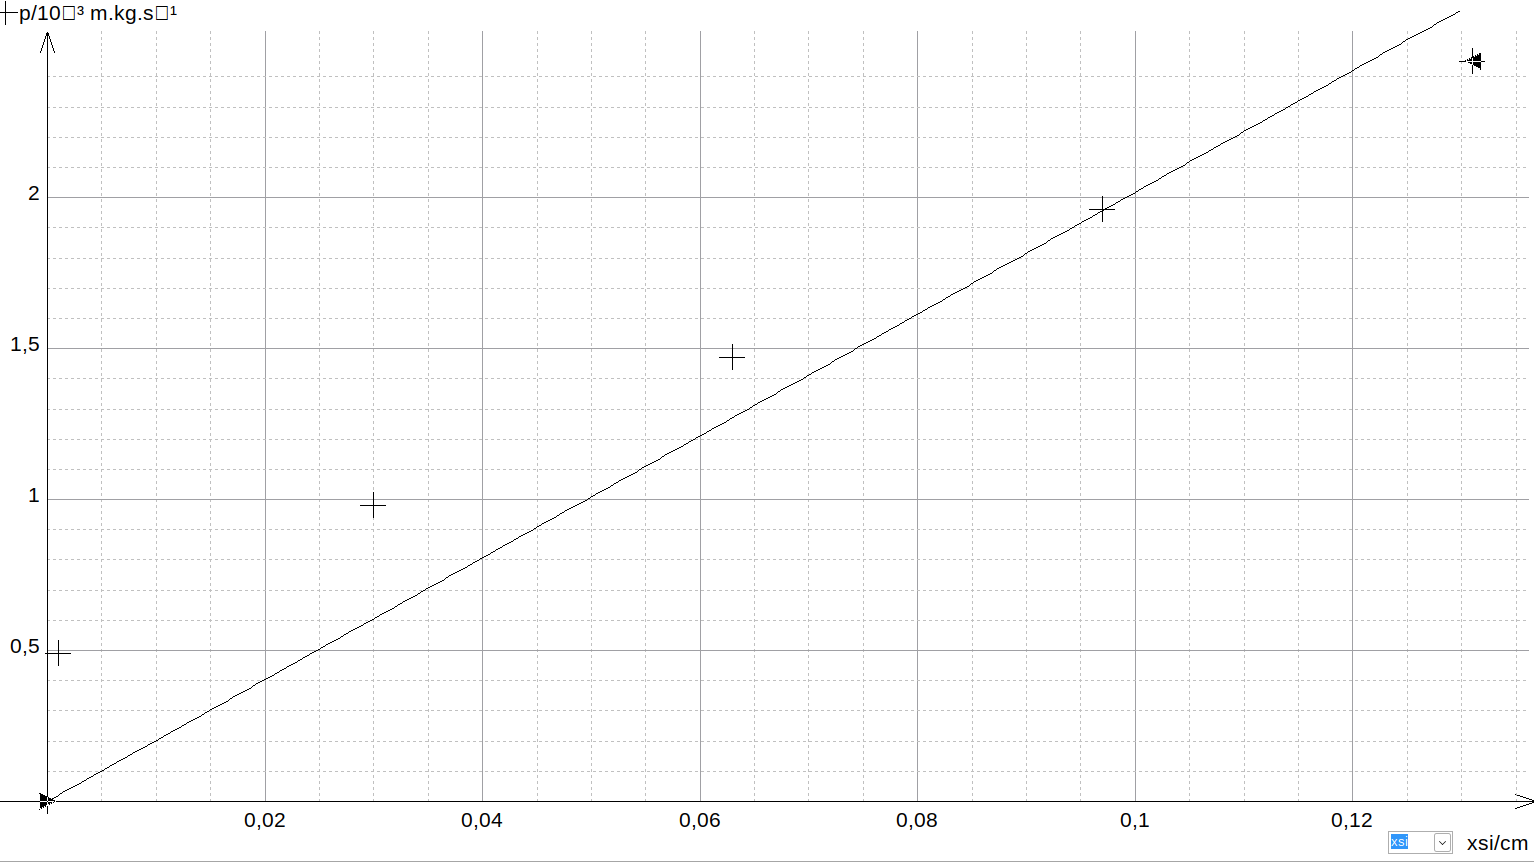
\includegraphics[scale=0.3]{R1_statique}
 \caption{Graphique obtenu avec le ressort 1. La droite modélisée est supperposée aux points obtenus}
\end{figure}
\newpage
\subsection{Approche dynamique}
\begin{figure}[H]
 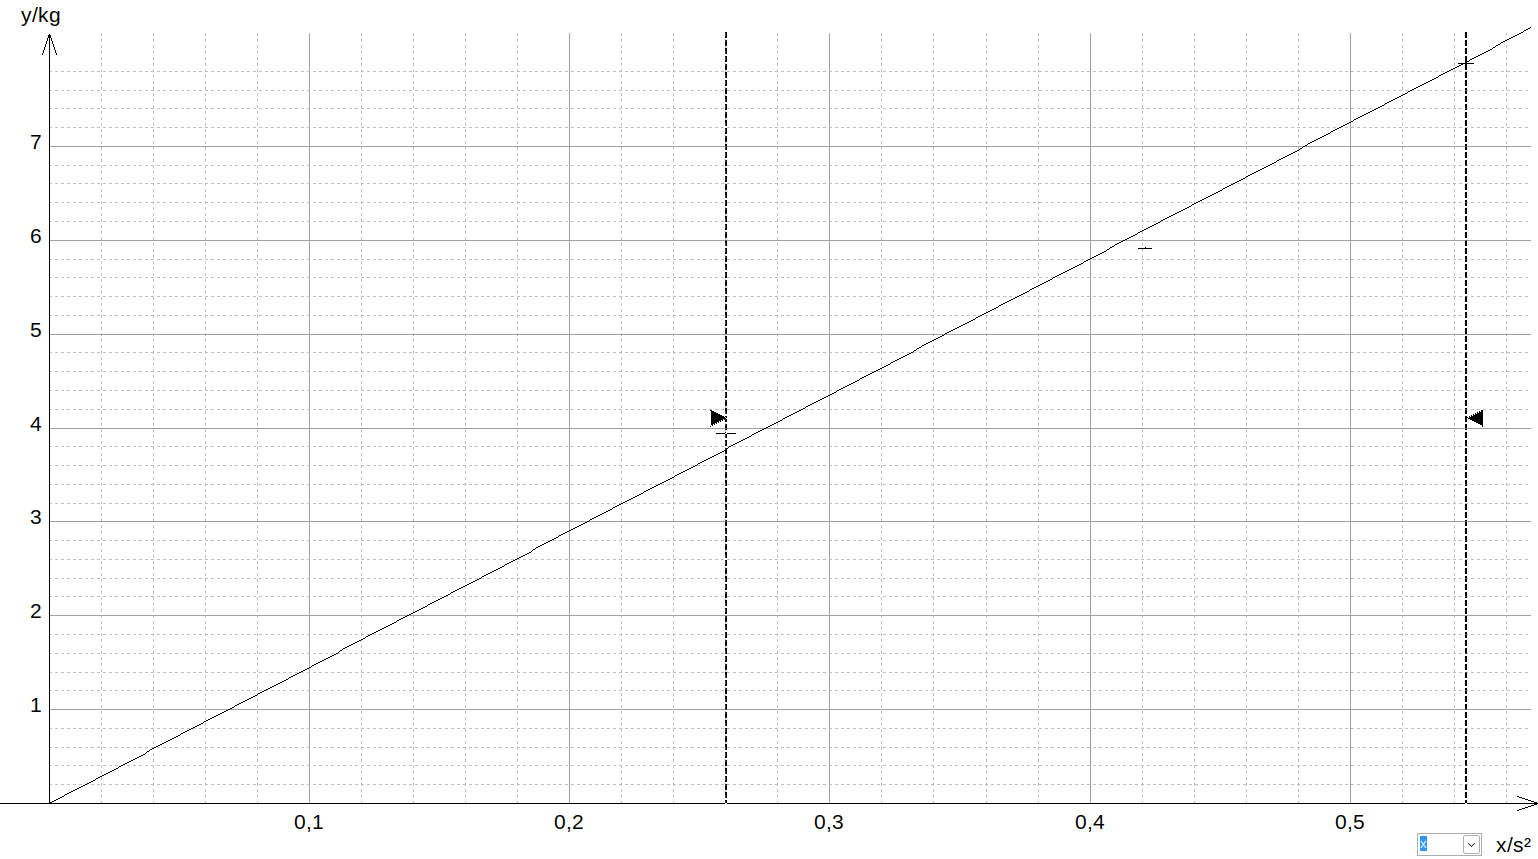
\includegraphics[scale=0.3]{R1_dyna}
 \caption{Graphique obtenu avec le ressort 1. La droite modélisée est supperposée aux points obtenus}
\end{figure}
\section{Exploitation des résultats}
\subsection{Approche statique}
Le système étant placé dans l'air, on néglige la poussée d'archimède par rapport aux deux autres forces que sont le poids et la force de rappel du ressort. Au moment de la mesure, le système est à l'équilibre. On peut donc écrire \[m_ig-kX_i = 0\] avec \(m_i\) la masse utilisée et \(X_i\) l'alongement correspondant. On connait toutes les grandeurs de cette expression sauf \(k\) que l'on cherche à déterminer. Pour ce faire, on peut tracer le graphe reliant le poids grandeurs à l'alongement : \[m_i g = kX_i\]. On trouvera une fonction linéaire dont le coeffciient directeur nous donnera la constante de raideur recherchée.

En traçant le graphe dans regressi, on obtient bien une fonction linéaire comme indiqué en figure 1. On déduit de la modélisation de regressi dans chaque cas la valeur de la constante de raideur avec un intervalle de confiance de 95\%  :
\begin{center}
\begin{tabular}{ll}
Ressort & Constante de raideur (\(N\cdot m^{-1}\))\\
1 & \(20.2\pm 1.7\)\\
2 & \(31.0\pm 6\)\\
3 & \(53.6\pm3.7\)
\end{tabular}
\end{center}

\subsection{Approche dynamique}
On peut exprimer la période T des oscillations en fonction de la masse utilisée et de la constante de raideur des ressorts. En effet, \[T = 2\pi \sqrt{\frac{m}{k}}\] On déduit de cette relation que \[4\pi^2m = kT^2\]. On va donc tracer \(4\pi^2m\) en fonction de \(T^2\) pour déterminer k, qui sera le coeffcient directeur de la droite. Avec un intervalle de confiance de 95\%, on obtient :

\begin{center}
\begin{tabular}{ll}
Ressort & Constante de raideur (\(N\cdot m^{-1}\))\\
1 & \(14.51\pm 0.23\)\\
2 & \(21.5\pm 2.3\)\\
3 & \(41.1\pm0.25\)
\end{tabular}
\end{center}

\section{Conclusion}
Les 2 méthodes donnent des résulats différents, mais du m\^eme ordre de grandeur. Il est d'environ 10 \(N\cdot m^{-1}\) pour les ressorts 2 et 3 et de 5 \(N\cdot m^{-1}\) pour le premier ressort. Cet écart peut \^etre du à des erreurs de manipulation lors de la deuxième manipulation. En effet, nous avons négligé la temps de réaction de l'expérimentateur et l'oscillation imparfaite du ressort. La première méthode semble plus fiable puisqu'elle introduit moins d'incertitude dans les mesures.

Il faudrait donc refaire la seconde méthode de façon à réduire l'incertitude sur la mesure de la période d'ooscillations, en filmant le pendule, puis en analysant la vidéo obtenue avec les programmes de traitement vidéo adaptés. Cela permettrait d'enlever l'incertitude liée au temps de réaction et de coordination de l'expérimentateur.
\end{document}
